\documentclass[sigconf,nonacm]{acmart}
\settopmatter{printacmref=false,printfolios=true}
\setcopyright{none}
\renewcommand\footnotetextcopyrightpermission[1]{}
\usepackage{amsmath,tabularx,array,enumitem,balance,tikz}
\usetikzlibrary{arrows.meta,positioning,shapes.geometric}
\definecolor{CourseBlue}{HTML}{315EFB}
\definecolor{CourseTeal}{HTML}{14877D}
\definecolor{CourseInk}{HTML}{18324A}
\hypersetup{colorlinks=true,linkcolor=CourseBlue,citecolor=CourseTeal,urlcolor=CourseTeal}
\newcolumntype{Y}{>{\raggedright\arraybackslash}X}
\setlist{leftmargin=*,topsep=3pt,itemsep=2pt}
\newcommand{\CourseNumber}{COMSCI/ECON 206}
\newcommand{\CourseName}{Computational Microeconomics}
\newcommand{\CourseSession}{Autumn 2026 Session 1}
\newcommand{\Instructor}{Professor Luyao Zhang}
\newcommand{\TeamCode}{FP10}
\newcommand{\SymposiumSession}{Pending course assignment}
\newcommand{\GitHubLink}{\href{https://github.com/micL1222/gt-tools-demos/tree/f9523b0fdd3f5dc4739dd1f08fe1265e049c1271/ps2_memory_portability}{snapshot \texttt{f9523b0}}}
\newcommand{\NotebookLink}{\href{https://colab.research.google.com/github/micL1222/gt-tools-demos/blob/f9523b0fdd3f5dc4739dd1f08fe1265e049c1271/ps2_memory_portability/notebooks/02_social_choice_mechanism_auction.ipynb}{Phase 3 Colab}}
\newcommand{\HuggingFaceLink}{\href{https://huggingface.co/spaces/mickeystk/ps2-stay-or-switch-memory-portability}{public Static Space}}
\newcommand{\PosterLink}{Planned; no result claimed}
\newcommand{\coursemeta}{\noindent\textbf{Submission to:} \CourseNumber{} --- \CourseName.\\
\textbf{Course session:} \CourseSession. \textbf{Team:} \TeamCode. \textbf{Symposium:} \SymposiumSession.\\
\textbf{Course instructor:} \Instructor. \textbf{Assignment:} PS2 collaborative research proposal.\par\smallskip}
\title{Stay or Switch? Strategic Memory Portability in Competing AI Assistants}
\author{Yiqiao Liu (Mickey)}
\affiliation{\institution{Duke Kunshan University}\city{Kunshan}\country{China}}
\email{yl1081@duke.edu}
\renewcommand{\shortauthors}{Yiqiao Liu (Mickey)}

\newif\ifTeachingAnnotations
\TeachingAnnotationstrue
% Visible, printable teaching notes. The original ACM text area is unchanged.
% Use main.tex for the clean submission and annotated.tex for guidance.
\ifTeachingAnnotations
\usepackage{eso-pic,tikz}
\usepackage[most]{tcolorbox}
\definecolor{AnnReplace}{HTML}{245BB4}
\definecolor{AnnConnect}{HTML}{08756C}
\definecolor{AnnDevelop}{HTML}{79469C}
\definecolor{AnnInk}{HTML}{21324A}
\definecolor{AnnRail}{HTML}{F4F6FA}
\definecolor{AnnLine}{HTML}{D4DCE7}
\newsavebox{\AnnRailBox}
\newcommand{\AnnNote}[4]{%
  \begin{tcolorbox}[enhanced,sharp corners,boxrule=0pt,frame hidden,
    colback=#2!5!white,borderline west={2pt}{0pt}{#2},
    left=7pt,right=7pt,top=5pt,bottom=5pt,before skip=6pt,after skip=0pt]
    \sffamily\fontsize{9.4}{11.8}\selectfont\color{AnnInk}\raggedright
    {\color{#2}\bfseries #1\quad #3}\par\vspace{2pt}#4
  \end{tcolorbox}}
\newcommand{\AnnPin}[4]{%
  \node[rounded corners=2bp,fill=#2,text=white,inner xsep=4bp,
    inner ysep=2.5bp,font=\sffamily\bfseries\fontsize{8}{9}\selectfont]
    at (#3,#4) {#1};}
\newcommand{\AnnPageTitle}{%
  \ifcase\value{page}\or
    Keep the PS1 structure\or
    Integrate evidence and impact\or
    Preserve the appendix sequence\or
    Update the same cumulative map\or
    Add only the PS2 extension record\else
    Continue the documented draft\fi}
\newcommand{\AnnPageNotes}{%
  \ifcase\value{page}\or\AnnNote{R1}{AnnReplace}{Replace team identity, not course identity}{%
Replace the title, team code, symposium session, member names, and emails. Keep the course, term, and \textbf{Course instructor: Professor Luyao Zhang}. The instructor is metadata, not a paper author.}

\AnnNote{R2}{AnnReplace}{Adapt the LaTeX-native teaser}{%
Edit \texttt{figures/ps2\_teaser.tex}. Keep the three evidence panels and synthesis logic, but replace their content with your actors, model, computation, behavioral test, A0-poster claim, and real-world case.}

\AnnNote{C1}{AnnConnect}{Keep the familiar five-section spine}{%
Section 1 asks the connected questions. Sections 2--4 answer the economics, computation, and behavior questions. Section 5 states the integrated contribution and practical impact. Carry the same claims into Appendix E.}

\AnnNote{D1}{AnnDevelop}{Choose the correct solution concept}{%
Define players, strategies, timing, information, beliefs, and payoffs before naming an equilibrium. Translate the same problem through game theory, social choice, and mechanism design; show what changes.}
\or
    \AnnNote{C2}{AnnConnect}{Make behavioral evidence consequential}{%
Use self-reflection and peer play to probe an assumption. State the competing explanation and the observation that would make the team retain, qualify, or revise the model, algorithm, or interface.}

\AnnNote{D2}{AnnDevelop}{Connect the real-world case to evidence}{%
Identify stakeholders, feasible benefit, risk, missing evidence, and correction route. Compare the standards of academia, industry, and public institutions without claiming impact that has not been measured.}

\AnnNote{R3}{AnnReplace}{Use the confirmed dates}{%
Review-ready: September 27 at 11:00 P.M. Symposium, peer evaluation, and practical-impact discussion: September 28. Final revision: September 30 at 11:00 P.M., before the October 1--2 holiday.}
\or\AnnNote{R4}{AnnReplace}{Credit people and work accurately}{%
Keep Professor Luyao Zhang as course instructor. Acknowledge peers, discussants, partners, data, software, adapted materials, and AI assistance only when used. Give each author an inspectable intellectual decision and output.}

\AnnNote{D3}{AnnDevelop}{Appendices A and B remain familiar}{%
Appendix A holds technical details, reproducibility, and AI disclosure. Appendix B retains the PS1 change record: earlier claim, dated evidence or feedback, revision, and intellectual consequence.}

\AnnNote{C3}{AnnConnect}{Appendices C and D preserve continuity}{%
Appendix C records open-source inspirations and the three-lens stress test. Appendix D preserves review, response, rerun, and revision. Do not replace missing feedback with invented evidence.}
\or
    \AnnNote{R5}{AnnReplace}{Complete the same eight rows}{%
Appendix E deliberately retains the PS1 structured abstract. Replace each prompt, save the prior version, and use complete, specific sentences.}

\AnnNote{C4}{AnnConnect}{Rows 1--4 must match Sections 1--3}{%
Use the same gap, application, connected questions, actors, incentives, timing, information, baseline, and evidence status. A reader should not encounter a different model in the table.}

\AnnNote{D4}{AnnDevelop}{Rows 5--8 close the evidence loop}{%
Separate actual and expected results. Explain the integrated intellectual merit and bounded practical impact. Record the dated feedback, revision location, verification, and consequence.}
\or\AnnNote{D5}{AnnDevelop}{Record the auction, not only the outcome}{%
State values or signals, prediction, bid, allocation, payment, stopping rule, utility, revenue, efficiency, behavioral observation, and revision for each treatment.}

\AnnNote{C5}{AnnConnect}{Check parity across three artifacts}{%
GitHub, Hugging Face, and the A0 poster must describe the same question, model, evidence status, result, and limits. The labels describe evidence perspectives, not fixed team roles.}

\AnnNote{D6}{AnnDevelop}{Use the symposium to revise}{%
Retain the September 28 poster and reviews. Record Keep, Revise, or Investigate decisions, rerun the affected check, and identify the exact September 30 change.}
\else
    \AnnNote{D}{AnnDevelop}{Return to the clean driver}{Use \texttt{main.tex} for submission. Recheck the two-page main limit and preserve supporting evidence in the appendices.}
  \fi}
\newcommand{\AnnPagePins}{%
  \ifcase\value{page}\or
    \AnnPin{R1}{AnnReplace}{31}{88}
    \AnnPin{R2}{AnnReplace}{31}{370}
    \AnnPin{C1}{AnnConnect}{31}{510}
    \AnnPin{D1}{AnnDevelop}{581}{400}
  \or
    \AnnPin{C2}{AnnConnect}{31}{94}
    \AnnPin{D2}{AnnDevelop}{31}{240}
    \AnnPin{R3}{AnnReplace}{581}{340}
  \or
    \AnnPin{R4}{AnnReplace}{31}{105}
    \AnnPin{D3}{AnnDevelop}{31}{390}
    \AnnPin{C3}{AnnConnect}{581}{240}
  \or
    \AnnPin{R5}{AnnReplace}{31}{92}
    \AnnPin{C4}{AnnConnect}{31}{260}
    \AnnPin{D4}{AnnDevelop}{31}{420}
  \or
    \AnnPin{D5}{AnnDevelop}{31}{92}
    \AnnPin{C5}{AnnConnect}{31}{310}
    \AnnPin{D6}{AnnDevelop}{581}{260}
  \fi}
\AddToHook{shipout/before}{\global\pdfpagewidth=912bp\relax}
\AddToShipoutPictureBG{\AtPageUpperLeft{%
  \begin{tikzpicture}[overlay,x=1bp,y=-1bp]
    \fill[AnnRail] (612,0) rectangle (912,792);
    \draw[AnnLine,line width=.6bp] (612,0)--(612,792);
  \end{tikzpicture}}}
\AddToShipoutPictureFG{\AtPageUpperLeft{%
  \savebox{\AnnRailBox}{\normalfont\begin{minipage}[t]{266bp}\AnnPageNotes\end{minipage}}
  \begin{tikzpicture}[overlay,x=1bp,y=-1bp]
    \AnnPagePins
    \node[anchor=north west,inner sep=0,text width=266bp] at (629,26) {%
      \sffamily\color{AnnInk}\fontsize{10}{12}\selectfont\raggedright
      \textbf{PS2 / ANNOTATED WORKING COPY}\par\vspace{5pt}
      {\fontsize{15}{17}\selectfont\bfseries\AnnPageTitle}\par\vspace{7pt}
      {\fontsize{9}{11}\selectfont
      \textcolor{AnnReplace}{\textbf{R REPLACE}}\quad
      \textcolor{AnnConnect}{\textbf{C CONNECT}}\quad
      \textcolor{AnnDevelop}{\textbf{D DEVELOP}}}};
    \node[anchor=north west,inner sep=0] at (629,102) {\usebox{\AnnRailBox}};
    \node[anchor=north west,inner sep=0,text width=266bp] at (629,748) {%
      \sffamily\fontsize{8.4}{10.2}\selectfont\color{AnnInk}
      Guidance is scaffolding. Submit from \texttt{main.tex}.
      \textbf{\thepage/5}};
  \end{tikzpicture}}}
\fi


\begin{document}
\begin{teaserfigure}
\captionsetup{skip=8pt}
\centering
\resizebox{\textwidth}{!}{%
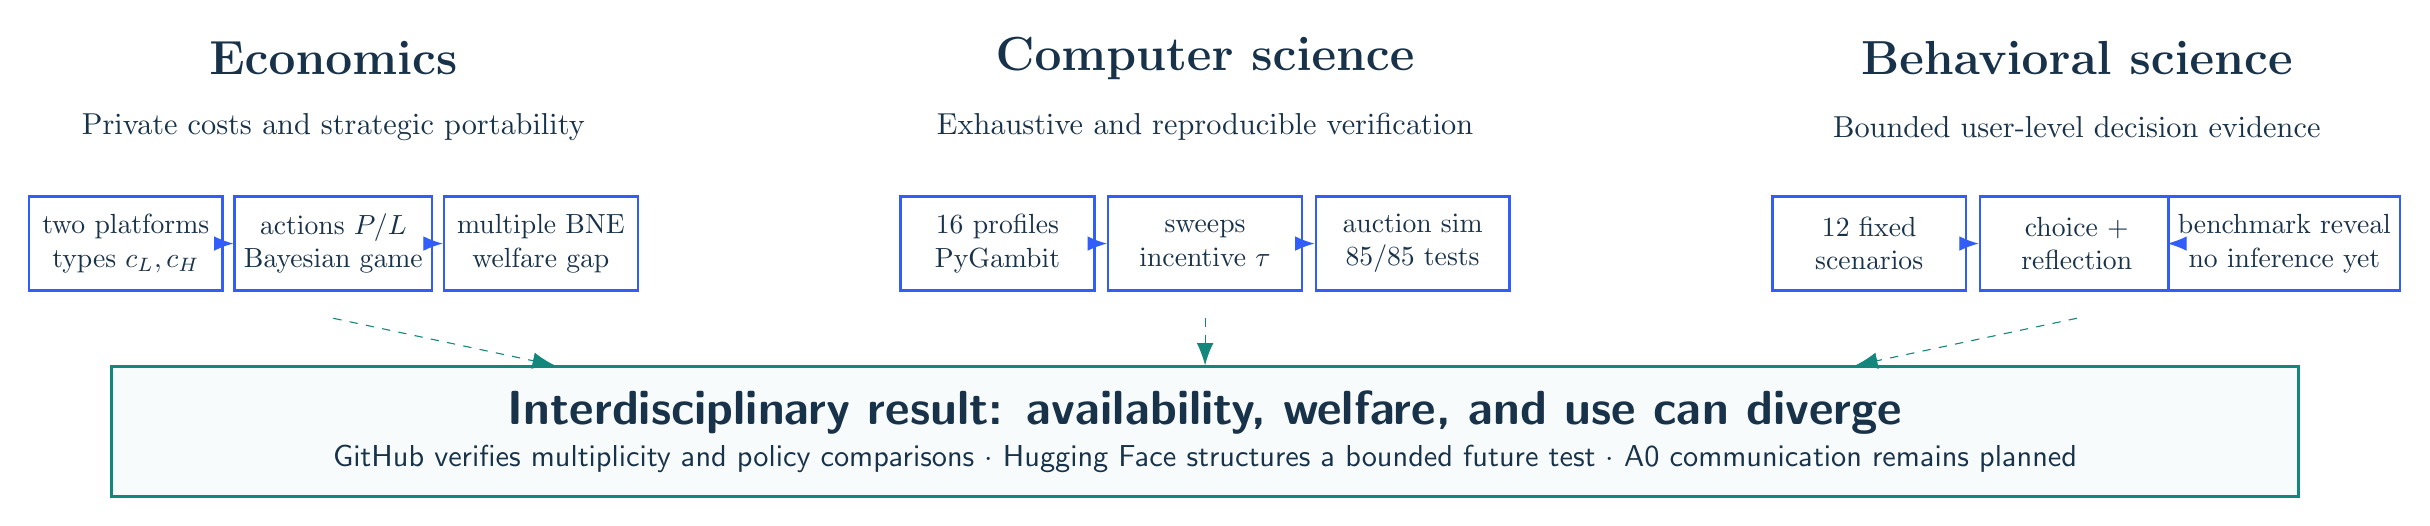
\begin{tikzpicture}[x=1pt,y=1pt,font=\sffamily,>=Latex]
\tikzset{
  heading/.style={font=\bfseries\fontsize{17}{19}\selectfont,text=CourseInk,align=center},
  label/.style={font=\fontsize{11}{13}\selectfont,text=CourseInk,align=center},
  mini/.style={draw=CourseBlue,line width=0.9pt,minimum width=70pt,minimum height=34pt,align=center,text=CourseInk,fill=white,font=\fontsize{10}{12}\selectfont},
  synthesis/.style={draw=CourseTeal,line width=1.1pt,minimum width=790pt,minimum height=47pt,align=center,text=CourseInk,fill=CourseTeal!3}
}
\node[heading] at (140,170) {Economics};
\node[label] at (140,145) {Private costs and strategic portability};
\node[mini] (e1) at (65,103) {two platforms\\types $c_L,c_H$};
\node[mini] (e2) at (140,103) {actions $P/L$\\Bayesian game};
\node[mini] (e3) at (215,103) {multiple BNE\\welfare gap};
\draw[CourseBlue,-{Latex[length=7pt]}] (e1)--(e2);
\draw[CourseBlue,-{Latex[length=7pt]}] (e2)--(e3);

\node[heading] at (455,170) {Computer science};
\node[label] at (455,145) {Exhaustive and reproducible verification};
\node[mini] (c1) at (380,103) {16 profiles\\PyGambit};
\node[mini] (c2) at (455,103) {sweeps\\incentive $\tau$};
\node[mini] (c3) at (530,103) {auction sim\\85/85 tests};
\draw[CourseBlue,-{Latex[length=7pt]}] (c1)--(c2);
\draw[CourseBlue,-{Latex[length=7pt]}] (c2)--(c3);

\node[heading] at (770,170) {Behavioral science};
\node[label] at (770,145) {Bounded user-level decision evidence};
\node[mini] (b1) at (695,103) {12 fixed\\scenarios};
\node[mini] (b2) at (770,103) {choice +\\reflection};
\node[mini] (b3) at (845,103) {benchmark reveal\\no inference yet};
\draw[CourseBlue,-{Latex[length=7pt]}] (b1)--(b2);
\draw[CourseBlue,-{Latex[length=7pt]}] (b2)--(b3);

\node[synthesis] (s) at (455,35) {\textbf{\fontsize{16}{18}\selectfont Interdisciplinary result: availability, welfare, and use can diverge}\\[3pt]
\fontsize{11}{13}\selectfont GitHub verifies multiplicity and policy comparisons $\cdot$ Hugging Face structures a bounded future test $\cdot$ A0 communication remains planned};
\draw[CourseTeal,dashed,-{Latex[length=8pt]}] (140,76)--(220,59);
\draw[CourseTeal,dashed,-{Latex[length=8pt]}] (455,76)--(455,59);
\draw[CourseTeal,dashed,-{Latex[length=8pt]}] (770,76)--(690,59);
\end{tikzpicture}}

\caption{Evidence chain for strategic memory portability. The platform game, computation, welfare/incentive comparisons, and allocation analogy are completed at snapshot \texttt{f9523b0}. The public Stay/Switch artifact structures a separate user test; behavioral inference and the A0 poster remain planned.}
\Description{Three panels connect a Bayesian platform game, reproducible computational checks, and a public user-decision artifact to a synthesis: portability may be socially valuable yet strategically absent, while behavioral conclusions and the A0 poster remain future work.}
\label{fig:teaser}
\end{teaserfigure}
\maketitle\raggedbottom\coursemeta

\section{Three connected research questions and verified gap}
AI-assistant memory can create switching costs and lock-in~\cite{farrell2007coordination}; portability can reduce that friction, but effects depend on the market~\cite{viard2007switching,kim2026portability}. Prior work models strategic compatibility in complementary products~\cite{jeon2023compatibility}. This project instead asks when two platforms with private implementation costs supply memory portability, whether strategic adoption matches a stated collective objective, and whether users would actually switch.

\textbf{Q1---Economics:} Which type-contingent portability choices are Bayesian equilibria, and how do welfare and a verified-portability incentive compare? \textbf{Q2---Computation:} Do exhaustive checks, sweeps, and an allocation analogy reproduce the thresholds? \textbf{Q3---Behavior:} When a benchmark favors switching, does persistence reflect status quo or omitted trust, privacy, and personalization? The shared question is when portability becomes both supplied and useful. Figure~\ref{fig:teaser} separates completed platform evidence from the planned user test.

\section{Answer to Q1: incentives and strategic model}
Nature independently draws each platform's private cost $c_i\in\{c_L,c_H\}$ with $\Pr(c_i=c_L)=p$; platforms simultaneously choose Portable ($P$) or Locked ($L$). With rival portability probability $q$,
\[
EU(P\mid c_i)=3q-1-c_i,\qquad EU(L\mid c_i)=q,
\]
so $P$ is a weak best response iff $2q-1\ge c_i$~\cite{harsanyi1968}. At $c_L=.2,c_H=1.2,p=.7$, type-level checks yield exactly two pure BNE, $(LL,LL)$ and $(PL,PL)$, plus a symmetric mixed equilibrium: high types lock and low types choose $P$ with probability $6/7$. Multiplicity is not resolved.

\emph{Game theory} gives the $PL$ threshold $p\ge(1+c_L)/2=.6$. \emph{Social choice} adds the cardinal objective $W=u_A+u_B+U_{user}$: at mobility value $m=1$, $W_{LL}=0$, $W_{PL}=2.17$, and the non-equilibrium comparator $W_{PP}=4$. \emph{Mechanism design} adds benefit $\tau$, changing the threshold to $p\ge(1+c_L-\tau)/2$. At $p=.4$, $\tau=.4$ sustains $PL$, but $LL$ remains a weak BNE through $\tau=1.2$: the intervention expands equilibria without selecting one.

\section{Answer to Q2: computation, auction comparison, and artifacts}
Python enumerates all $4\times4=16$ pure profiles and checks every type against deviations; an independent PyGambit Harsanyi game returns the same two pure BNE. Integer-built grids sweep $p=.01,\ldots,.99$, $c_L=0,.05,\ldots,1.15$, and $\tau=0,.05,\ldots,2.5$. Saved CSV/JSON includes rejected profiles; 85/85 tests pass.

The allocation analogy assigns one primary-assistant slot between two iid $U[0,1]$ platform values. Portability lowers the assumed reserve from $r=.5$ to $r=.2$. Second price uses truthful bids~\cite{vickrey1961counterspeculation}; first price uses $b(v;r)=(v^2+r^2)/(2v)$ for $v\ge r$. With seed 20603 and 100,000 common draws, allocation rises from .75193 (analytical .75) to .96004 (.96). Locked/portable unconditional payments are .41788/.36320 (first price) and .41818/.36414 (second price); conditional efficiency is one. The user is not auctioned, reserves are normalized assumptions, and no optimal-auction claim is made~\cite{myerson1981optimal}.

\textbf{GitHub:} \GitHubLink. \textbf{Notebook:} \NotebookLink.\\
\textbf{Hugging Face:} \HuggingFaceLink. \textbf{A0 poster:} \PosterLink.

\clearpage\balance
\section{Answer to Q3: behavior and interdisciplinary integration}
The public Static Space crosses hurdles $r=.20$, $.35$, or $.50$ with benefits $g=.15$, $.30$, $.45$, or $.60$. A user decides before seeing the rule, rates switching difficulty, personalization loss, privacy, and trust, then sees the simplified benchmark ``Switch iff $g>r$'' and decides again. Six scenarios predict Stay and six Switch. Status-quo-bias evidence motivates the hypothesis of persistence~\cite{samuelson1988statusquo}, but a Stay choice can instead reflect preferences omitted from $g-r$. The Space has no backend, tracking, persistent store, or cross-browser aggregation; peer summaries use prior plays in the current page session only. It is publicly deployed and technically verified, but no participant-level conclusion is claimed.

A future structured classroom test would compare initial/final decisions and ratings across the fixed scenarios. Persistence concentrated when $g-r>0$, conditional on measured concerns, would qualify the user-mobility term; sensitivity to disclosure would motivate interface revision. Benchmark alignment would retain the simple rule only as a descriptive classroom benchmark. Either result would leave platform BNE as a separate unit of analysis.

\section{Advanced development, real-world impact, and roadmap}
Harsanyi's incomplete-information foundation and the Vickrey--Myerson auction literature discipline the economic claims; reproducible enumeration makes every profile inspectable. The distinctive contribution is an auditable chain from privately costly platform portability, through welfare and incentives, to user mobility---while keeping firm equilibria, simulated allocations, and prospective behavioral evidence separate.

Consider a student or writer deciding whether to move years of AI-assistant context. Users may gain choice; incumbent and entrant platforms face implementation, competition, and security incentives; regulators and institutions need interoperable, privacy-preserving standards. Academia requires identification and replicable evidence, industry requires reliability and security tests, and public institutions require access, accountability, and correction. The next discriminating test is whether portable-memory scenarios increase actual switching relative to no-portability scenarios without raising privacy concern; the present artifact does not answer it.

\begin{table}[h]\caption{From foundations to an interdisciplinary contribution.}\small
\begin{tabularx}{\columnwidth}{@{}p{1.35cm}Y@{}}\toprule
\textbf{Horizon}&\textbf{Milestone and evidence}\\\midrule
Foundation&Incomplete-information games; switching costs; auction design.\\
PS2&Two pure BNE, welfare/incentive comparisons, seeded allocation simulation, public decision artifact.\\
Symposium&Planned A0 claim and genuine peer challenges; none recorded yet.\\
Next study&Consent-based scenario comparison with privacy and access safeguards.\\
2056&Validated interoperable-memory institutions with accountable correction.\\\bottomrule
\end{tabularx}\end{table}

\noindent\textbf{Expected 2056 Nobel Prize and Turing Award contribution statement.}
By 2056, the aspiration is a tested theory and computational design for interoperable AI memory that aligns platform incentives with user agency. Progress would require multi-market validation, secure standards, mechanism trials, and behavioral evidence; neither awards nor impact are predicted by PS2.

\subsection*{Open Science Statement}
Snapshot \texttt{f9523b0} contains source, two executed notebooks, pinned dependencies, deterministic outputs, tests, and evidence boundaries. From \path{ps2_memory_portability/}, run \texttt{conda run -n cs206-ps2 python -m unittest discover -s tests -v}; the recorded result is 85/85. The Static Space is public; it stores no shared participant dataset. The repository has no new blanket license grant. The poster remains planned.

\subsection*{Statement of Contribution to the UN's SDGs}
No demonstrated SDG impact is claimed. A future secure portability standard could be evaluated against SDG target 9.1's inclusive-infrastructure objective~\cite{un_sdg} using successful export/import, accessibility, privacy incidents, and switching completion as indicators. Possible harms include data leakage and exclusion when transferred context is incomplete; audits and user-controlled correction are required.

\subsection*{Submission milestones}
Review-ready: September 27, 2026, 11:00 P.M. Beijing time. Symposium and peer evaluation: September 28, 2:45--5:15 P.M., IB 2050. Final revision: September 30, 11:00 P.M. Beijing time. No symposium or peer-review outcome is reported in this review-ready version.

\clearpage\nobalance
\section*{Author Notes}
\subsection*{Acknowledgements}
\textbf{Course instructor: Professor Luyao Zhang.} The author acknowledges the official COMSCI/ECON 206 PS2 Overleaf Student Template, the open-source Python and LaTeX tools identified in Appendix~C, and permitted assistance from OpenAI Codex as disclosed in Appendix~A.1. No PS2 peer, discussant, symposium, community-partner, or classroom-auction contribution had been received by this review-ready version; none is invented or attributed. The author remains responsible for the proposal and remaining errors.

\subsection*{Team and individual contributions}
\textbf{Joint contribution statement (solo team; 124 words).} This solo project links a static Bayesian game of privately costly memory portability to three inspectable extensions: a cardinal social-welfare comparator, a verified-portability incentive, and a reserve-based platform-allocation analogy. Its contribution is the separation of three questions often conflated in portability debates: whether firms strategically supply portability, whether modeled outcomes rank differently under a stated collective objective, and whether users switch when technical friction falls. Reproducible enumeration, PyGambit agreement, deterministic sweeps, seeded auction simulation, and 85 automated tests verify the formal claims. A public Static Space implements twelve hypothetical Stay/Switch scenarios while explicitly providing no persistent participant dataset. The paper therefore offers an integrated, falsifiable research design and public artifacts, not an empirical claim about firms, users, welfare, or status-quo bias.

\textbf{Yiqiao Liu (Mickey), sole and first author.} Liu selected the memory-portability question; approved the private-cost Bayesian structure, normalized payoffs, welfare objective, verified-portability intervention, auction mapping, and behavioral evidence boundary; and is accountable for interpreting every result. Inspectable outputs are in \url{ps2_memory_portability/}, especially the two notebooks, \url{outputs/}, the public Space, and this paper source. Verification includes direct/PyGambit agreement, analytical thresholds, scenario parity, public deployment checks, 85/85 tests, and LaTeX/PDF audits. The official team code is FP10. The next responsibility is to confirm the symposium session, create the A0 poster from its official template, obtain genuine September 28 reviews, and record Keep/Revise/Investigate decisions without delegating personal reflection to AI.

\bibliographystyle{ACM-Reference-Format}\bibliography{references}

\appendix
\section{Technical details and reproducibility}
\label{app:technical}
\subsection{Model, timing, and type-level verification}
Platforms $A,B$ independently draw $c_i\in\{.2,1.2\}$ with $\Pr(c_i=.2)=.7$, observe only their own type, and simultaneously choose $P$ or $L$. Normalized own payoff is $2-c_i$ under $(P,P)$, $-1-c_i$ under $(P,L)$, $1$ under $(L,P)$, and $0$ under $(L,L)$. Thus
\[
\begin{aligned}
EU(P\mid c)&=3q-1-c, & EU(L\mid c)&=q,\\
P\in BR(c)&\Longleftrightarrow 2q-1\ge c.&&
\end{aligned}
\]
A pure strategy is a complete type map in $\{LL,PL,LP,PP\}$. The checker evaluates every type of both players in all 16 profiles; zero-probability endpoints are excluded from the full-support sweep.

\begin{table}[h]
\caption{Predetermined parameters and evidence status.}
\begin{tabularx}{\columnwidth}{@{}p{2.3cm}Y@{}}\toprule
\textbf{Component}&\textbf{Value and status}\\\midrule
Platform benchmark&$c_L=.2,c_H=1.2,p=.7$; normalized, not estimated.\\
Pure BNE&$(LL,LL)$, $(PL,PL)$; no asymmetric pure BNE at benchmark.\\
Mixed candidate&High types lock; low types use $P$ with $x^*=6/7$.\\
Social choice&$W=u_A+u_B+U_{user}$; cardinal comparability assumed.\\
Mechanism&$EU_\tau(P\mid c)=3q-1-c+\tau$; mechanism cost unmodeled.\\
Auction&$N=100{,}000$, seed 20603, iid $U[0,1]$, reserves .5/.2.\\
Behavior&12 fixed scenarios; zero participant-level results.\\\bottomrule
\end{tabularx}
\end{table}

\subsection{Language-independent verification procedure}
\begin{enumerate}
\item Load the predetermined cost, prior, mobility, incentive, reserve, and seed values.
\item For each ordered pair of type-contingent strategies, compute the rival-induced $q$; for each positive-probability type, compare the prescribed action with its deviation. Save every accepted and rejected profile.
\item Cross-check benchmark pure BNE with a separately constructed PyGambit Harsanyi game; fail if sets differ.
\item Sweep integer-built $p,c_L,\tau,m$ grids; compare classifications with analytical thresholds before plotting.
\item Draw one seeded valuation sample; reuse it for first-/second-price and locked/portable conditions; compare simulated $1-r^2$, payment, utility, and efficiency.
\item Run all tests, execute notebooks from clean kernels, validate the behavioral catalog, and compare paper claims with saved JSON/CSV fields.
\end{enumerate}

\subsection{Verified outputs and limitations}
At $m=1$, $W_{LL}=0$, $W_{PL}=2.17$, and $W_{PP}=4$; $PP$ is a comparator, not a Phase 2 BNE. For symmetric $PL$, $p\ge(1+c_L-\tau)/2$, while the high type locks only when $\tau\le1+c_H-2p$. At $p=.4$, the minimum $\tau$ for weak $PL$ is .4. At $p=.7$, $LL$ remains weak through $\tau=1.2$, and $PP$ first appears weakly at $\tau=.2$. No welfare-optimal $\tau$ is claimed.

The auction's analytical allocation probability is $1-r^2$. The saved simulation gives .75193 at $r=.5$ and .96004 at $r=.2$, with absolute errors .00193 and .00004. The same valuation draws are used throughout; 400,000 raw in-memory rows are not committed, and a deterministic 400-row sample is retained. The application does not auction a person, calibrate AI markets, or implement a Myerson-optimal mechanism.

The recorded environment is Python 3.12.14, NumPy 2.3.5, SciPy 1.17.0, pandas 2.2.3, matplotlib 3.10.8, PyGambit 16.7.0, nbformat 5.11.1, nbclient 0.11.0, and ipykernel 7.3.0. Reproduce from repository snapshot \texttt{f9523b0}:
\begin{verbatim}
cd ps2_memory_portability
conda run -n cs206-ps2 python scripts/run_phase2.py
conda run -n cs206-ps2 python scripts/run_phase3.py
conda run -n cs206-ps2 python -m unittest \
  discover -s tests -v
\end{verbatim}
Expected test result: 85 passed, 0 skipped, 0 failures, 0 errors. The two tracked notebooks are executed artifacts, not substitutes for the source modules.

The public Static Space revision is \texttt{9ffb3ca} (full revision recorded in the audit). It has no backend, analytics, cookies, or persistent browser storage; refreshing or closing clears its page-session aggregate. The review-ready A0 poster does not yet exist and is not misreported as an output.

\subsection{AI-use disclosure}
OpenAI Codex (GPT-5 family, September 23--26, 2026) assisted with repository inspection, Python implementation and debugging, test design and execution, notebook and visualization construction, literature-source checking, the Gradio and Static Space artifacts, LaTeX drafting, compilation, and evidence/parity audits. Significant instructions required preserving the research question and official template, separating actual from planned evidence, and prohibiting fabricated author, peer, auction, symposium, and participant records. Suggestions that would overstate empirical evidence, infer missing metadata, or treat the user as literally auctioned were rejected. The author supplied or approved the research direction and remains responsible for every modeling choice, citation, interpretation, and final submission. Automated tests and artifact comparisons are recorded; personal reflection, peer review, and final human approval must be completed by the author.

\section{Cumulative Intellectual Development}
PS1 studied costly information acquisition before a collective AI decision: two agents chose Research or Skip, producing a free-riding benchmark and a reproducible NashPy check. PS2 does not claim topic continuity. It retains the methodological lesson that strategic interdependence, solution concept, computation, and behavioral evidence must be separated, then applies it to a new shared question: privately costly portability between competing AI assistants.

\begin{table}[h]
\caption{Dated development record; no peer-review cause is inferred.}
\begin{tabularx}{\columnwidth}{@{}p{1.6cm}p{1.85cm}Y@{}}\toprule
\textbf{Date / evidence}&\textbf{Revision}&\textbf{Intellectual consequence}\\\midrule
PS1 final, Sept. 2026&Costly Research/Skip benchmark with future behavior test&Established model-first and actual/planned evidence discipline.\\
Sept. 24, commit \texttt{796bee4}&Private-cost $P/L$ Bayesian game&Made implementation cost private and BNE the correct solution concept.\\
Sept. 24, \texttt{181c840}&Added welfare, $\tau$, and auction comparison&Exposed equilibrium--welfare tension and a bounded policy lever.\\
Sept. 25, \texttt{7a2e02e}&Verified literature claims&Narrowed compatibility, portability, and status-quo claims to supported analogies.\\
Sept. 26, \texttt{f9523b0}&Public Static Space verified&Separated technical deployment from participant evidence.\\\bottomrule
\end{tabularx}
\end{table}

The author initially focused on whether portability is supplied. The welfare comparison showed that $PP$ can rank highest without being a benchmark equilibrium; the mechanism sweep showed that an incentive can add portability equilibria while lock-in persists; and the behavioral design showed that technical portability does not logically imply user switching. The current integrated claim is therefore conditional: platform adoption, collective desirability, feasible allocation, and user response are distinct propositions requiring distinct evidence.

\section{Open-source and three-lens inspiration}
\begin{table}[H]
\caption{Software/source record and design consequence.}
\footnotesize
\begin{tabularx}{\columnwidth}{@{}p{1.65cm}p{1.75cm}Y@{}}\toprule
\textbf{Source / tool}&\textbf{Version / license}&\textbf{Capability, limit, consequence}\\\midrule
Python ecosystem&Versions in App.~A; upstream licenses apply&Deterministic analysis; package behavior is environment-dependent.\\
PyGambit&16.7.0; GPL-2.0-or-later&Independent pure-BNE cross-check; direct checker remains authoritative.\\
Gradio&6.28.0; upstream license&Local prototype; free hosted compute was unavailable, prompting static conversion.\\
HTML/CSS/JS&Browser-native&Public zero-build artifact; no shared response store.\\
ACM \texttt{acmart}&Official course-bundled class&Required paper layout; content does not imply ACM publication.\\
Course repository&Public; no new blanket license grant&Inspectable evidence; public availability is not additional reuse permission.\\\bottomrule
\end{tabularx}
\end{table}

The three lenses produce different decisions. Game theory asks which type-contingent strategies survive unilateral deviation. Social choice adds users and a declared collective objective, revealing a contested cardinal-comparability assumption. Mechanism design changes the action payoff through $\tau$, then tests adoption and equilibrium-selection limits. None of these establishes observed firm conduct. The auction comparison tests a separate allocation analogy; the behavioral Space tests a separate user-level decision rule.

Literature is used only for the general mechanisms it supports: switching costs and lock-in~\cite{farrell2007coordination}, strategic compatibility~\cite{jeon2023compatibility}, setting-specific portability competition~\cite{viard2007switching}, security trade-offs~\cite{kim2026portability}, status-quo motivation~\cite{samuelson1988statusquo}, and auction foundations~\cite{vickrey1961counterspeculation,myerson1981optimal}. Their parameters and outcomes are not transferred to AI assistants.

\newpage
\section{Review response and revision record}
\label{app:review}
This document is the review-ready v1 due September 27, before the September 28 symposium. No PS2 peer review, discussant comment, instructor comment, classroom-auction observation, or symposium question had been received when it was compiled. Therefore no substantive Keep/Revise/Investigate decision is attributed to another person. The prior PS1 record concerns a different topic and is historical development evidence, not direct review of this proposal.

\begin{table}[h]
\caption{Review-ready status; empty evidence is reported, not filled.}
\footnotesize
\begin{tabularx}{\columnwidth}{@{}p{1.55cm}p{1.55cm}Y@{}}\toprule
\textbf{Required record}&\textbf{Current status}&\textbf{Next verified action}\\\midrule
Review-ready v1&Complete&Retain PDF, ZIP, commit, and audit as baseline.\\
Two peer reviews&Not yet received&After Sept. 28, record named/dated forms and exact claims.\\
Discussant / instructor&None received for PS2&Record only comments actually delivered.\\
Author decision&Pending evidence&Classify each consequential comment Keep, Revise, or Investigate.\\
Rerun/final v2&Not yet applicable&Rerun affected test and cite changed file/location for Sept. 30.\\\bottomrule
\end{tabularx}
\end{table}

The pre-review parity audit did produce author-side corrections: it preserved the two pure-BNE wording, labeled $PP$ a welfare comparator, separated Static page-session aggregation from participant evidence, and labeled the poster and classroom observations as pending. These are verification edits, not peer feedback.

\clearpage\onecolumn
\section{Structured abstract and cumulative proposal map}\label{app:abstract}
\begin{table}[H]
\caption{Appendix E structured abstract; actual and planned evidence remain separate.}
\label{tab:abstract-map}
\renewcommand{\arraystretch}{1.18}
\begin{tabularx}{\textwidth}{@{}p{0.27\textwidth}Y@{}}
\toprule
\textbf{Proposal element} & \textbf{Current statement / change} \\
\midrule
Background & AI assistants accumulate user-specific memory. Switching costs can create lock-in, while firms may make compatibility choices strategically. Existing work does not supply this project's static private-implementation-cost Bayesian result or AI-user evidence. \\
Motivation and application & A student or writer may want to move long-lived context between assistants. Users, incumbent and entrant platforms, regulators, and institutions face benefits from choice and risks from privacy, incomplete transfer, security, and unequal access. \\
Three connected questions & Economics asks when portability is a BNE, how it ranks under a collective objective, and how $\tau$ changes incentives. Computation asks whether exhaustive checks and allocation simulations reproduce thresholds. Behavior asks whether users switch when $g>r$. Together: when is portability supplied and practically useful for competitive mobility? \\
Method and model assumptions & Two privately informed platforms simultaneously choose $P/L$; $c_L=.2,c_H=1.2,p=.7$. Direct enumeration and PyGambit check BNE; deterministic sweeps test welfare and incentive thresholds; a seeded two-bidder allocation analogy compares first and second price at reserves .5/.2; twelve fixed scenarios structure future user evidence. \\
Results or expected results & \textbf{Actual:} pure BNE $(LL,LL)$, $(PL,PL)$; low-type mix $6/7$; $W_{PP}>W_{PL}>W_{LL}$ on the tested $m$ grid; $\tau$ expands portability equilibria without selecting one; allocation .75193/.96004; 85/85 tests; public Static Space. \textbf{Planned:} participant, classroom-auction, poster, symposium, and causal evidence. \\
Intellectual merits & The project shows that strategic availability, modeled collective value, feasible allocation, and user adoption are distinct claims. Combining analytical thresholds, exhaustive computation, and a bounded behavioral design prevents one evidence type from standing in for another. \\
Practical impacts & Potential value is user mobility and contestability; risks include privacy loss, partial transfer, manipulation, and exclusion. No impact is demonstrated. Future evaluation should measure successful transfer, switching, access, and incidents, with user-controlled correction and independent audit. \\
Feedback received and revision made & No PS2 peer or symposium feedback had been received in review-ready v1. The author-side parity audit narrowed claims, preserved Gradio failure history, recorded successful Static deployment and team code FP10, and marked the session, poster, classroom play, and future review as pending. The prior PS1 topic is preserved as methodological history, not evidence for PS2. \\
\bottomrule
\end{tabularx}
\end{table}
\noindent The prior PS1 structured abstract concerned costly information acquisition before collective decisions. Its retained methodological lesson is explicit separation of formal prediction, computation, and uncollected behavior; its substantive results are not reused as memory-portability evidence.

\clearpage\twocolumn
\section{PS2 extension record: auction, linked artifacts, poster, and symposium}
\subsection{Auction laboratory record}
The completed evidence is a seeded computational benchmark, not a classroom play. Each treatment uses two iid $U[0,1]$ private platform values, one primary-assistant slot, one sealed bid per platform, Platform A tie-breaking, a reserve, allocation to the highest eligible bid, mechanism-specific payment, and termination after one allocation decision.

\begin{table}[h]
\caption{Completed simulation treatments; $N=100{,}000$, seed 20603.}
\begin{tabularx}{\columnwidth}{@{}p{1.15cm}rrrr@{}}\toprule
&\textbf{$r$}&\textbf{Alloc.}&\textbf{Pay.}&\textbf{Eff.}\\\midrule
First, locked&.50&.75193&.41788&1.00\\
First, portable&.20&.96004&.36320&1.00\\
Second, locked&.50&.75193&.41818&1.00\\
Second, portable&.20&.96004&.36414&1.00\\\bottomrule
\end{tabularx}
\end{table}

First-price eligible bids follow $b(v;r)=(v^2+r^2)/(2v)$; second-price bids equal value. ``Eff.'' is conditional efficiency given allocation. Utilities and conditional payments are preserved in \url{outputs/auction_summary.csv}. \textbf{Classroom record:} no game URL, assigned value/signal, planned bid, actual bid/outcome, payment, utility, revenue, behavioral observation, or resulting revision was available. Those fields must be completed only after genuine play.

\subsection{Linked-artifact parity}
\begin{tabularx}{\columnwidth}{@{}p{1.55cm}Y@{}}\toprule
\textbf{Artifact}&\textbf{Verified parity status}\\\midrule
GitHub&Snapshot \texttt{f9523b0}; same private-cost game, inputs, formulas, outputs, 85 tests, and limitations.\\
Hugging Face&Same user-level Stay/Switch question, 12 scenarios, $g>r$ rule, no participant conclusion, page-session privacy boundary.\\
A0 poster&Not yet created. It must reuse the shared question, actual results, real-world case, limits, instructor, acknowledgements, and artifact links; no parity claim is made yet.\\\bottomrule
\end{tabularx}

\subsection{Symposium and practical-impact record}
This review-ready package predates the September 28 symposium. No presentation version, peer-evaluation form, question, or Keep/\allowbreak Revise/\allowbreak Investigate response exists yet. For the concrete migration case, affected parties are users, incumbent and entrant assistants, institutions procuring AI, and regulators. Potential benefit is safer competitive mobility; risks are leakage, degraded context, strategic misrepresentation, and inaccessible transfer. Missing evidence includes real implementation costs, security performance, transfer fidelity, switching choices, and distributional effects. Proposed correction routes are user-controlled export/import, data minimization, provenance logs, deletion and rollback, accessibility testing, complaint procedures, and independent audit. The September 30 record must identify every actual change and rerun its affected check.

\end{document}
